\documentclass{article} % For LaTeX2e
\usepackage{nips15submit_e,times}
\usepackage{hyperref}
\usepackage{url}
\usepackage{booktabs}       % professional-quality tables
\usepackage{amsfonts}       % blackboard math symbols
\usepackage{nicefrac}       % compact symbols for 1/2, etc.
\usepackage{microtype}      % microtypography
\usepackage{amsmath}
\usepackage{caption}
\usepackage[ruled,vlined]{algorithm2e}
\usepackage{graphicx}
%\documentstyle[nips14submit_09,times,art10]{article} % For LaTeX 2.09


\title{Breaking News Bandits}


\author{Achille Aknin \& Alban Pierre}

% The \author macro works with any number of authors. There are two commands
% used to separate the names and addresses of multiple authors: \And and \AND.
%
% Using \And between authors leaves it to \LaTeX{} to determine where to break
% the lines. Using \AND forces a linebreak at that point. So, if \LaTeX{}
% puts 3 of 4 authors names on the first line, and the last on the second
% line, try using \AND instead of \And before the third author name.

\newcommand{\fix}{\marginpar{FIX}}
\newcommand{\new}{\marginpar{NEW}}

%\nipsfinalcopy % Uncomment for camera-ready version

\begin{document}


\maketitle

\begin{abstract}
Multi-armed bandit (MAB) is a very common problems, studied with many different approachs.
Besides, it is also derived in many ways, such as adversarial bandit, non-stationary bandit or distributed bandit.
Here we focus on a variation called
Breaking News multi-armed bandit, when one arm can have suddenly a high reward : this arm stays hot for a time before it comes back to normal.
In this report, we describe a model of such MABs and then expose some algorithms to maximize the rewards
on Breaking News MABs, before testing it on our model.
\end{abstract}

\section{Introduction}

Among differences from the classic multi armed bandit, the expectation can become
very high compared to normal rewards, so an algorithm should keep pulling the same
arm if it is hot. When no arms is hot, the algorithm should pull each arm frequently
in order to find a new breaking new. But during that time, the algorithm should
also maximize its reward, because each arm does not hove the same 'normal' reward.
We implemented several algorithms that have similar behaviors : in the first
section, we explain data generation and then in second part the widely used
Thompson Sampling and Upper Confidence Bound algorithms. Then we focus on an
exact but very slow algorithm (GM) in part three. In section four we explain an
algorithm that tries to detect whether we have a hot state based on maximum/minimum
previous rewards and in the next part based on the previous rewards variance.
Then in part six and seven we moved on an algorithm based on nearest neighbors.
Eventually in the eight section we provide more results for different problems.
\newline

Note : the code we used in our experiments is in matlab (compatible with octave) and can be found at the address : https://github.com/alban-pierre/projet-RL-Breaking\_news\_bandit


\section{Data generation}

To generate the data, we model each arm to have several states, and for each state the reward follows a Gaussian distribution of a mean and a variance specific to that state (and to that arm). In the following experiments we used the means and variance :
\begin{center}
\begin{tabular}{rccc}
	Arms : & 1st & 2nd & 3rd \\
	Mean of the 1st state : & 2.0 & 3.0 & 1.0 \\
	Variance of the 1st state : & 1.0 & 1.0 & 1.0 \\
	Mean of the 2nd state : & 70.0 & 50.0 & 80.0 \\
	Variance of the 2nd state : & 1.0 & 1.0 & 1.0 \\
\end{tabular}
\end{center}
For the transition probabilities : when one arm is in a hot state, this arm has a probability $p=0.1$ to come back to normal, the others stay at a normal state. When each arm is at the normal state, then we sample one arm randomly and it became hot with probability $p=0.03$. In such a model, there are at most one arm in the hot state. An example of a generated data with these parameters is shown in figure 1.
\newline

\begin{figure}[h]
	\begin{center}
		%\framebox[4.0in]{$\;$}
		%\fbox{\rule[-.5cm]{0cm}{4cm} \rule[-.5cm]{4cm}{0cm}}
		%\includegraphics[width=1.0]{generated_data.png} TODO
	\end{center}
	\caption{Example of generated data}
\end{figure}

For the last section, we also used a model where several arms can become hot at the same time, with approximately the same probabilities of transition.

\section{Upper Confidence Bound Algorithm}

In this section, we recall the widely used Upper Confidence Bound (UCB) Algorithm,
as described in [1],
that seeks to optimize the reward in the case of a regular MAB problem. The main
idea is to compute an expected mean for each arm $\hat\mu_a(t)$, upper bounding it
by a confidence on the mean being high for arms that haven't been drawn often. We
then draw the arm with the highest upper bound.
This way we make sure that every arm is used from time to time.
\begin{equation*}
	a^* = argmax_{a} \Big(\hat\mu_a(t) + \sqrt{\frac{log(t)}{2N_a(t)}}\Big)
\end{equation*}

\begin{algorithm}
	\caption{UCB Algorithm}
	\For{$i=1:T_{max}$}{
		Compute $a^* = argmax_{a} \Big(\hat\mu_a(t) + \sqrt{\frac{log(t)}{2N_a(t)}}\Big)$\;
		Draw arm $a^*$ and receive reward $r(t)$\;
		Update $\hat\mu_{a^*}(t+1) = \frac{N_{a^*}(t)\times \hat\mu_{a^*}(t) + r(t)}{N_{a^*}(t)+1}$\;
		Update $N_{a^*} = N_{a^*}+1$\;
	}
\end{algorithm}

\section{Exact probabilities inference with Gaussian Mixture}

This first algorithm tries to be mathematically exact : we use a Gaussian mixture model using the Expectation-Maximisation algorithm to compute the mean of each state of each arm. Then given theses means (and variances) we compute the probability for each observed reward to come from one state. This gives for each state of each arm a sequence of probabilities. With theses sequence we compute the transition probabilities via a gradient descent. Thus, given the means and the transition probabilities, we can compute the expectation of each arm.
\newline

In practice, we add an exploration term to force the algorithm to explore, but even with that it does not lead to better results than Thompson-Sampling. The reason of that poor result is that when we compute the expectation of each arm, a little change in transition probabilities leads to a huge change in the expectation of an arm (at least if this arm was not seen for a few time).

Figure 3 show the exact expectation of an arm as a function of the time since the last draw. There are 2 curves for each arm because here each arm has 2 states (hot or not). Thus for one arm the upper curve is the expectation of that arm if the last time we draw it it was in the hot state, and the lower curve is the expectation of that arm if the last time we draw it it was in the normal state. The 2 curves converge because if we don't pull an arm for a long time, the probability to be hot is the same, whether it was hot or not the last time we draw that arm.

So in the case of the Gaussian Mixture algorithm, this is the plateau on the right that moves a lot due to approximations in transition probabilities, and then the outcome of the general algorithm is changed.

\begin{figure}[h]
	\begin{center}
		%\framebox[4.0in]{$\;$}
		%\fbox{\rule[-.5cm]{0cm}{4cm} \rule[-.5cm]{4cm}{0cm}}
		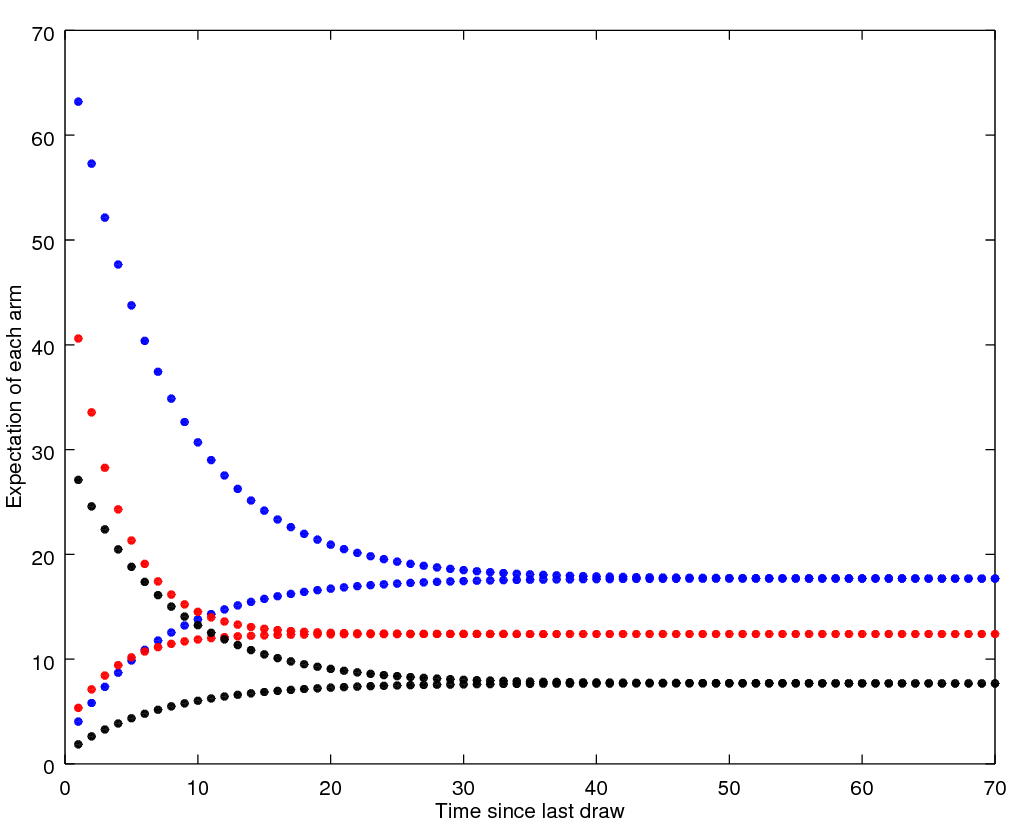
\includegraphics[width=1.0\textwidth]{expectations.png}
	\end{center}
	\caption{Expectation of each arm as a function of time since the last draw}
\end{figure}

Besides, this plot gives insight of what algorithms should do : if an arm is in the hot state, the expectation is high so this algorithm should pull the same arm over and over until it is not hot anymore. When this hot arms become normal, the other arms were not pulled since a long time, so we are far on the right for these arms. Then we should chose the one that has the highest plateau. If this arm is not hot, then the expectation of this arm falls back to the beginning of the curve (on the bottom left). The expectation of the last arm not drawn is still on the plateau (so relatively high compared to other arms) and we should pull that arm.

Note that if all arms are normal, this plot gives an optimal sequence of draws : as we select the highest point, the points not selected step by one unit on the right, thus increasing. And we repeat taking the highest point. Thus the arm with the lowest normal reward is not selected offenly since it has to increase more to become the highest point.

\section{UCB\_Var}

In this section, we describe an algorithm based on the UCB algorithm and on an estimation of the maximal
value that an arm can reach when it is not hot, and use this estimation to detect when the
arm is hot. Our purpose is then to estimated from a sequence of samples on a given arm $a$ the range
of values we expect the next sample to be in. We will then exploit the mean $\hat\mu_a(t)$ and variance $\hat\sigma_a(t)$
estimated from the previous samples and consider that if an arm stays in its initial
state, the reward drawn $r$ should be in the range $r \in [\hat\mu_a(t)-\hat\sigma_a(t), \hat\mu_a(t)+\hat\sigma_a(t)]$.

To take into account the uncertainty on both the mean and the range we might have,
we will add a term decreasing with the number of sample rewards we have on the arm $a$:
\begin{equation}\label{UCB-var-bound}
	r \in \Big[\hat\mu_a(t)-\hat\sigma_a(t)-\sqrt{\frac{1}{2N_a(t)}}, \hat\mu_a(t)+\hat\sigma_a(t)+\sqrt{\frac{1}{2N_a(t)}}\Big]
\end{equation}

The algorithm is then as follows: we proceed as in the UCB algorithm, and if at
some time $t$ we draw a sample from an arm and the reward obtained $r(t)$ is higher than the upper bound
in Eq.~\ref{UCB-var-bound}, we then consider that this arm is in a hot state.
We temporarily forget the samples we've seen for this arm, and continue
with $r(t)$ as the only reward observed so far for arm $a$. This has the effect
of having a bigger mean $\hat\mu(t+1) = r(t)$ and having $N_a(t+1) = 1$, making this arm more suceptible
to be drawn next time. If at some time $t'$, we observe a reward $r(t')$ lower
than the lower bound in Eq.~\ref{UCB-var-bound}, we then consider that this arm has
left the hot state, and proceed with the samples observed before time $t$, having
once again a smaller mean $\hat\mu(t')$.

In practice, this algorithm gets quite stable and good results if we make sure,
with some adaptations, to not keep thinking that an arm is hot when it is actually
not. The main drawback of this algorithm is that we need to remember each
reward observed observed at along, and compute its variance, and we can't avoid
a linear operation at each step, so the algorithm has a complexity of $\mathcal{O}(N^2)$ where N
is the number of steps.

\section{UCB\_Max}

To avoid the quadratic complexity of the previous algorithm, we choose to not compute
the actual variance $\hat\sigma_a(t)$, but instead simply remember the maximal value
observed on each arm $M_a(t)$ (and for a hot state, the minimal value $m_a(t)$).
At each step, we now check whether $r(t) > M_a(t)$ (or whether $r(t) < m_a(t)$ for a hot state),
and if it is the case then we consider that arm $a$ entered the hot state (or left the hot state)
and we reinitialise $\hat\mu_a(t)$ (or take back the old value).

This algorithm does not have results as good as UCB\_Var, but it faster and only have
a linear complexity, since computing the mean $\hat\mu_a(t)$ and the max $M_a(t)$
can be done with a finite number of operations at each step.

\section{Nearest Neighbors Upper Confidence Bound Algorithms}

Here we try to estimate the expectations shown in figure 2. Unlike the Gaussian Mixture algorithm, we will use here a Monte-Carlo estimation. So the Nearest Neighbors algorithm starts by choosing each arm twice (initialization) and then from each arm, it embeds all previous rewards of this arm in the space (Last reward of the arm; Time since last draw; Reward observed). In practice the rewards are shifted and resized to fit in $[0,1]$ and the time since last draw in rather $exp(-time since last draw)$ so that a time of 1 is far from a time of 2 but a time of 56 is right next to time of 57.

Then we compute where is the current point in that space - along the two first dimensions - and we take the average along the third dimension (expected reward) of all points that are within a distance of $d=0.1$. If there are no points in that range we take the nearest point. Then as we did it for each arm we choose the arm that has obtained the maximum average plus the upper confidence bound variance.

In practice this algorithm performs at most like the UCB algorithm, but if we take the average over the $K$ nearest neighbors instead of the points within a $d$ range, then we get very good results.

\section{K-Nearest Neighbors Long Term Expectation}

Let's go back to the figure 2 : it show the best arm to draw given the last reward and the time since last draw. Unfortunately, this plot gives the greedy algorithm only for the next draw. Indeed we can think of an algorithm that draws a hot arm over and over, and then that draws a second arm even if the first arm is still hot, just because the expectation of that second arm is not $p(hot)*reward(hot) + p(normal)*reward(normal)$ but $p(ho	t)*reward(hot)*10 + p(normal)*reward(normal)$ if the algorithm knows that the second arms keeps being hot for at least 10 iterations.

This is the problem we tried to fix in this algorithm : first it tries to approximate the expectation just like KNN, but after a non-negligible number of draws, we add in the expectation the second reward obtained, and then a little while after, the third rewards obtained, etc. We also add a decay rate so that the first reward counts more than following rewards.

In practice it does not yield to an improvement because the change in probabilities is little so it does not change rewards significantly.


\section{Time of computation and results other different arms settings}

Here we show the results of each algorithms presented in last sections on the multi armed bandit settings presented in the Data generation section :

\begin{figure}[h]
	\begin{center}
		%\framebox[4.0in]{$\;$}
		%\fbox{\rule[-.5cm]{0cm}{4cm} \rule[-.5cm]{4cm}{0cm}}
		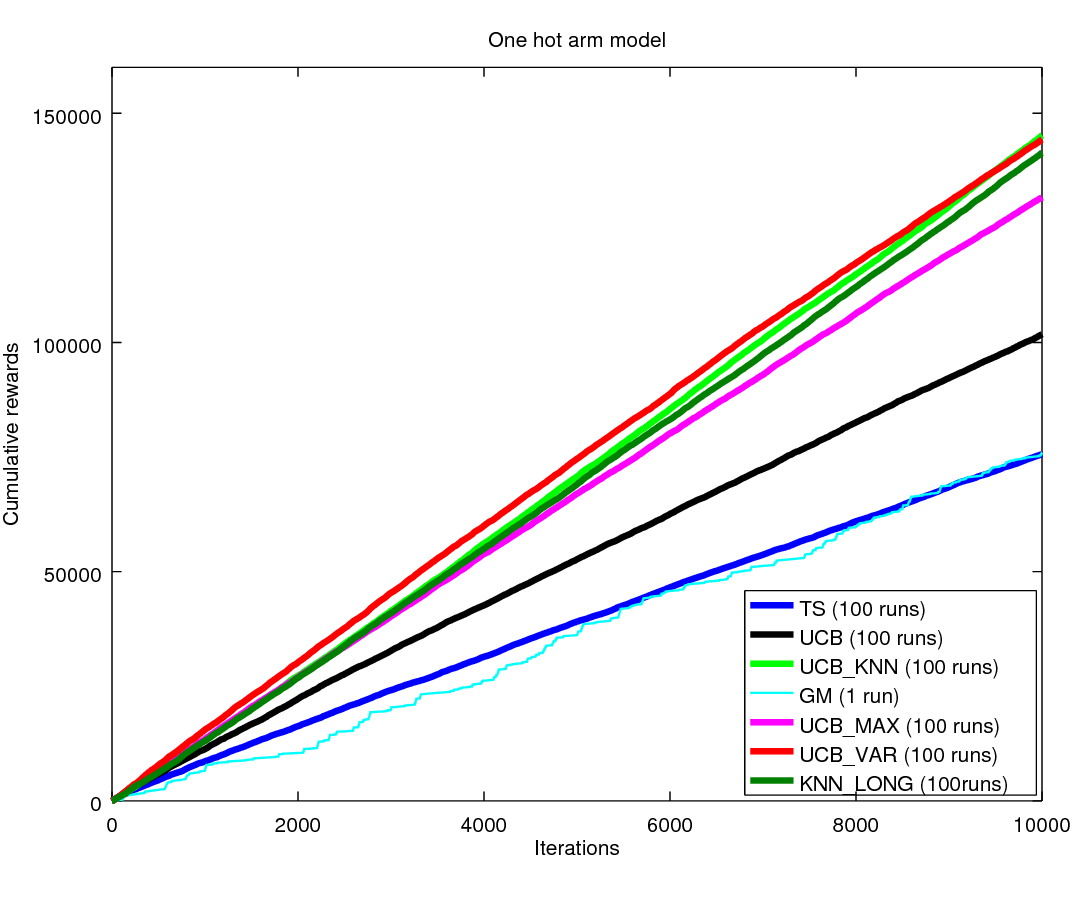
\includegraphics[width=1.0\textwidth]{all_10000it.png}
	\end{center}
	\caption{All algorithms for 10000 iterations (3 arms * 2 states, at most one hot arm)}
\end{figure}

\begin{figure}[h]
	\begin{minipage}[b]{.49\linewidth}
		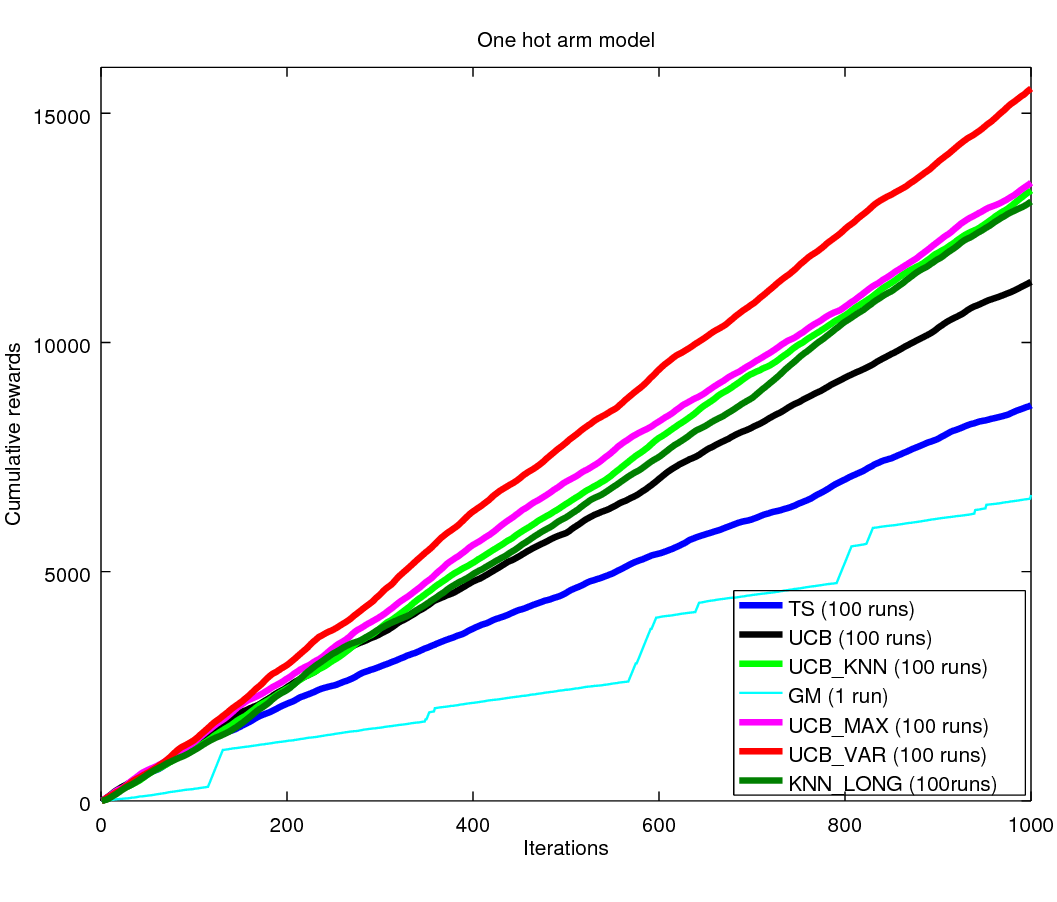
\includegraphics[width=1.0\textwidth]{begin_1000it.png}
		\caption{1000 first iterations (3*2, one)}
	\end{minipage}
	\hfill
	\begin{minipage}[b]{0.49\linewidth}
		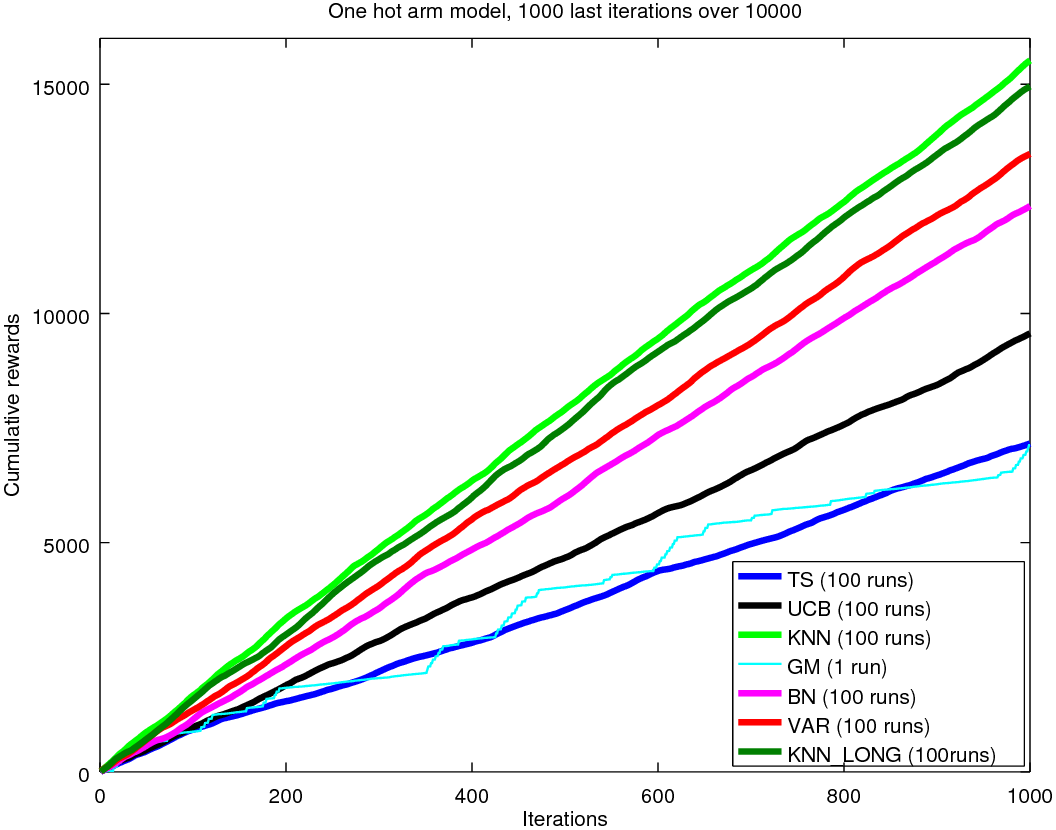
\includegraphics[width=1.0\textwidth]{last_1000it.png}
		\caption{1000 last iterations (3*2, one)}
	\end{minipage}
	\label{fig:f}
\end{figure}

Here are the computation time observed for 10000 iterations :
\begin{center}
	\begin{tabular}{rccccccc}
		Arms : & TS & UCB & GM & UCB\_KNN & KNN\_LONG & UCB\_MAX & UCB\_VAR \\
		Time (sec) : & 7.12 & 2.19 & 1000.5 & 25.39 & 35.85 & 3.06 & 5.37
	\end{tabular}
\end{center}

We can see that the performance of TS and UCB decrease over time, which is normal because they reduce exploration over time, and it is exploration that discovers hot states. The UCB\_KNN and KNN\_LONG increase their performance as theirs Monte-Carlo estimations are more and more precise. The UCB\_MAX and UCB\_VAR algorithms perform well in the beginning.

\clearpage
We also tried for data where several arms can become hot at the same time (with approximately the same transition probabilities, 5 runs each) :

\begin{figure}[h]
	\begin{center}
		%\framebox[4.0in]{$\;$}
		%\fbox{\rule[-.5cm]{0cm}{4cm} \rule[-.5cm]{4cm}{0cm}}
		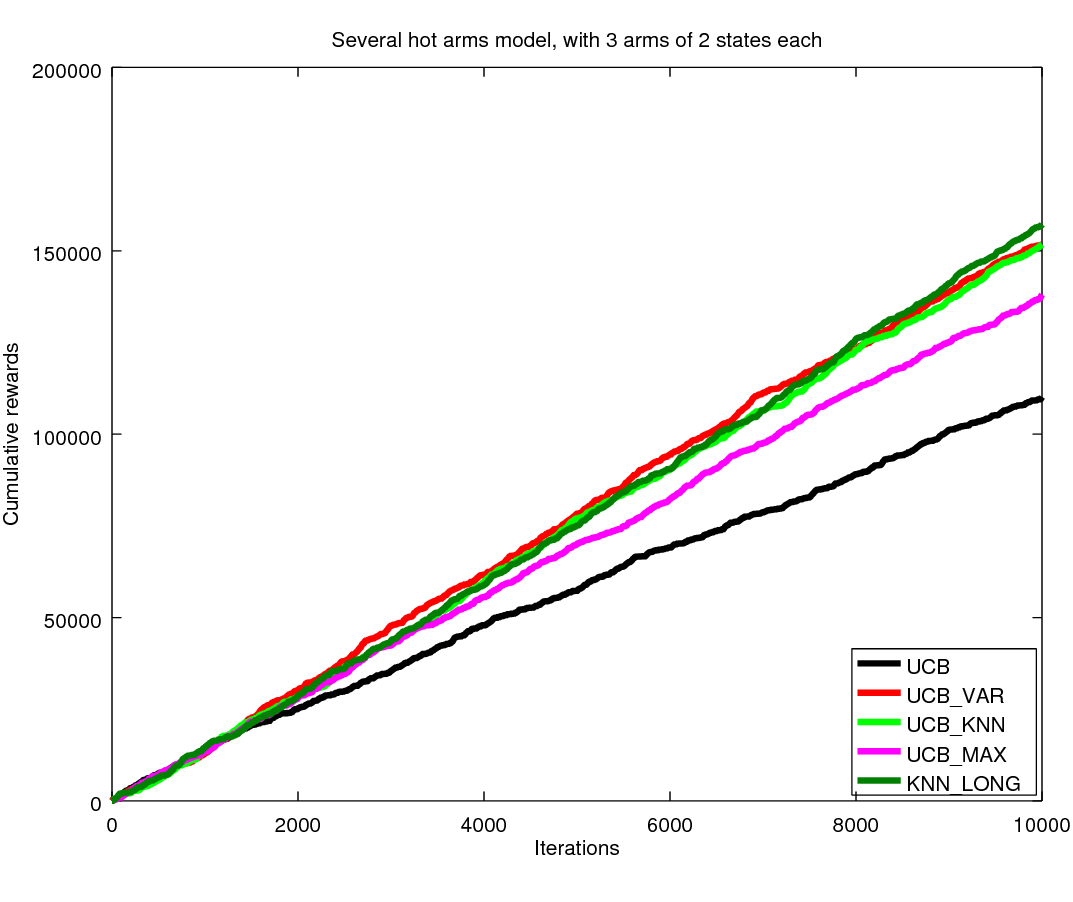
\includegraphics[width=1.0\textwidth]{all_m_10000it.png}
	\end{center}
	\caption{All algorithms for 10000 iterations (3 arms * 2 states, several hot arms)}
\end{figure}

\begin{figure}[h]
	\begin{minipage}[b]{.49\linewidth}
		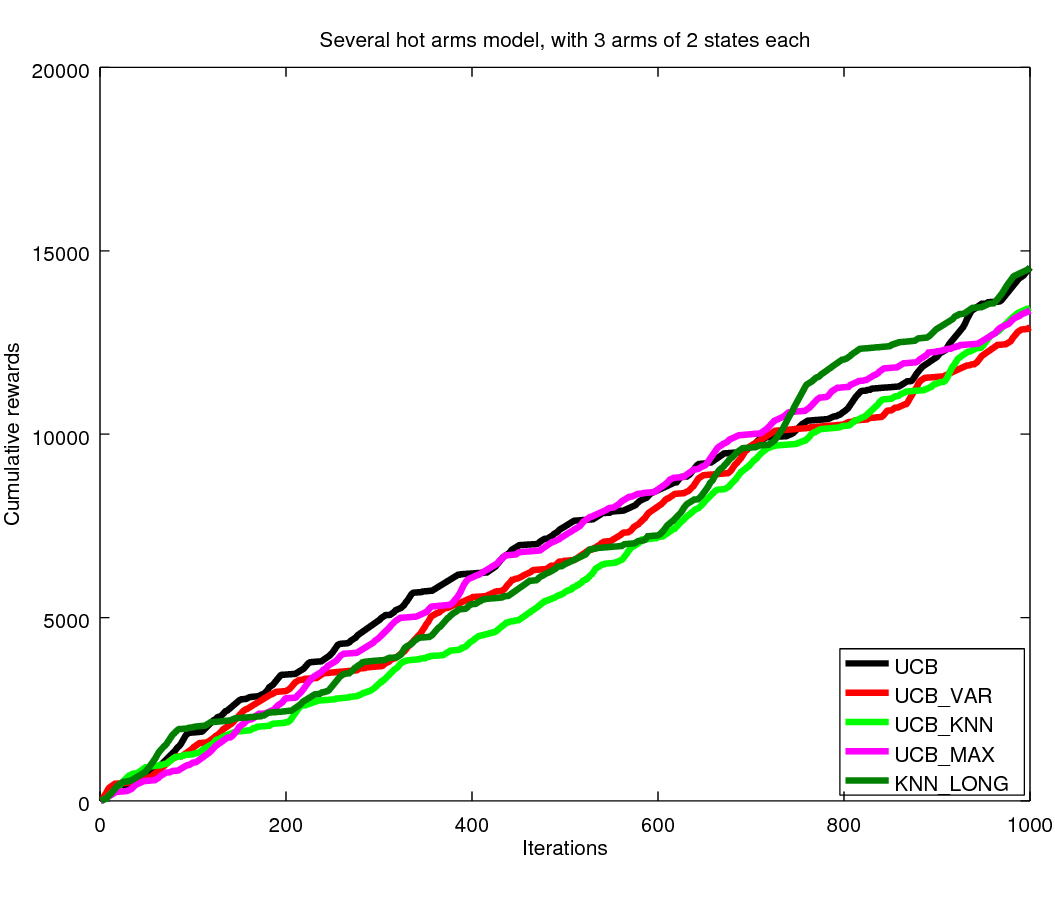
\includegraphics[width=1.0\textwidth]{begin_m_1000it.png}
		\caption{1000 first iterations (3*2, several)}
	\end{minipage}
	\hfill
	\begin{minipage}[b]{0.49\linewidth}
		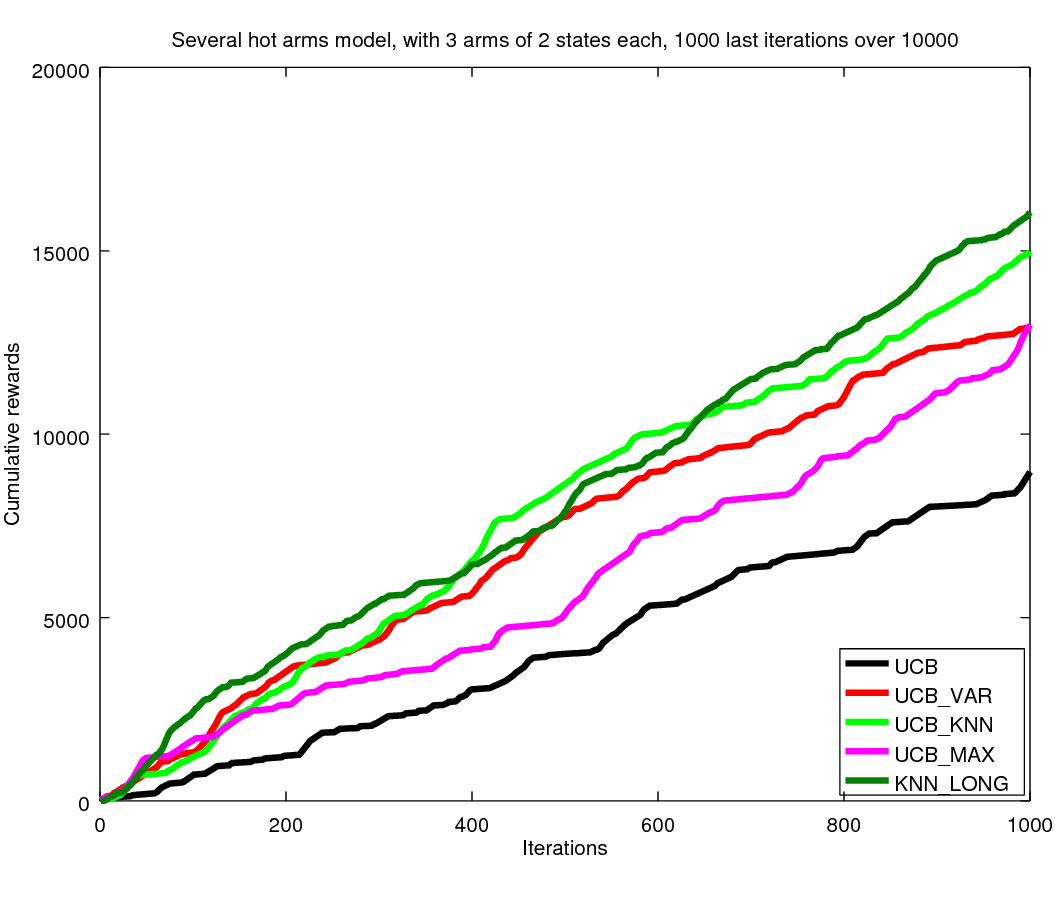
\includegraphics[width=1.0\textwidth]{last_m_1000it.png}
		\caption{1000 last iterations (3*2, several)}
	\end{minipage}
	\label{fig:f}
\end{figure}

We observe quite the same things except for KNN\_LONG : this algorithm sometimes tries different arms while they were on a hot arm with a comparatively low hot reward. The other algorithms keep hitting the same arm when it is hot, so they don't see the difference from the case where there are at most one hot arm.

\clearpage
Then we tried with 5 arms with 3 states each (with one hot arm at most, 10 runs each) : 

\begin{figure}[h]
	\begin{center}
		%\framebox[4.0in]{$\;$}
		%\fbox{\rule[-.5cm]{0cm}{4cm} \rule[-.5cm]{4cm}{0cm}}
		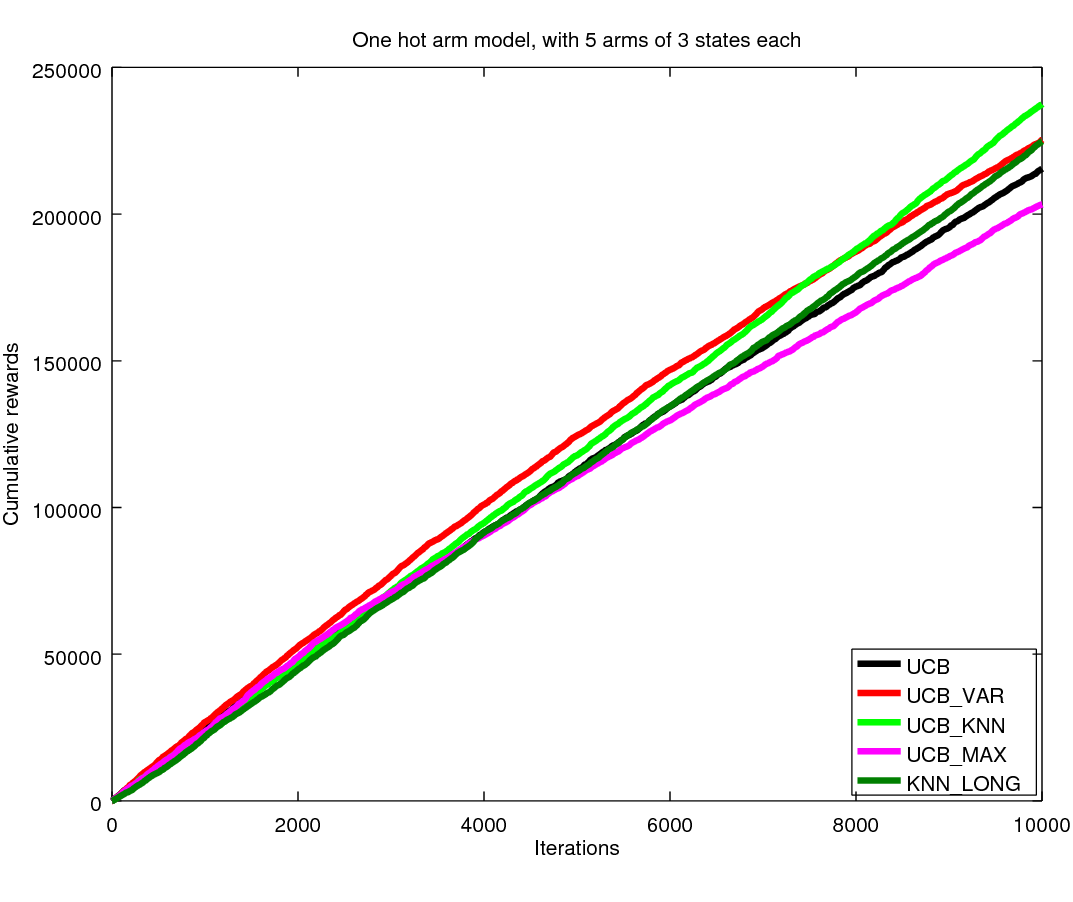
\includegraphics[width=1.0\textwidth]{all_s_10000it.png}
	\end{center}
	\caption{All algorithms for 10000 iterations (5 arms * 3 states, at most one hot arm)}
\end{figure}

\begin{figure}[h]
	\begin{minipage}[b]{.49\linewidth}
		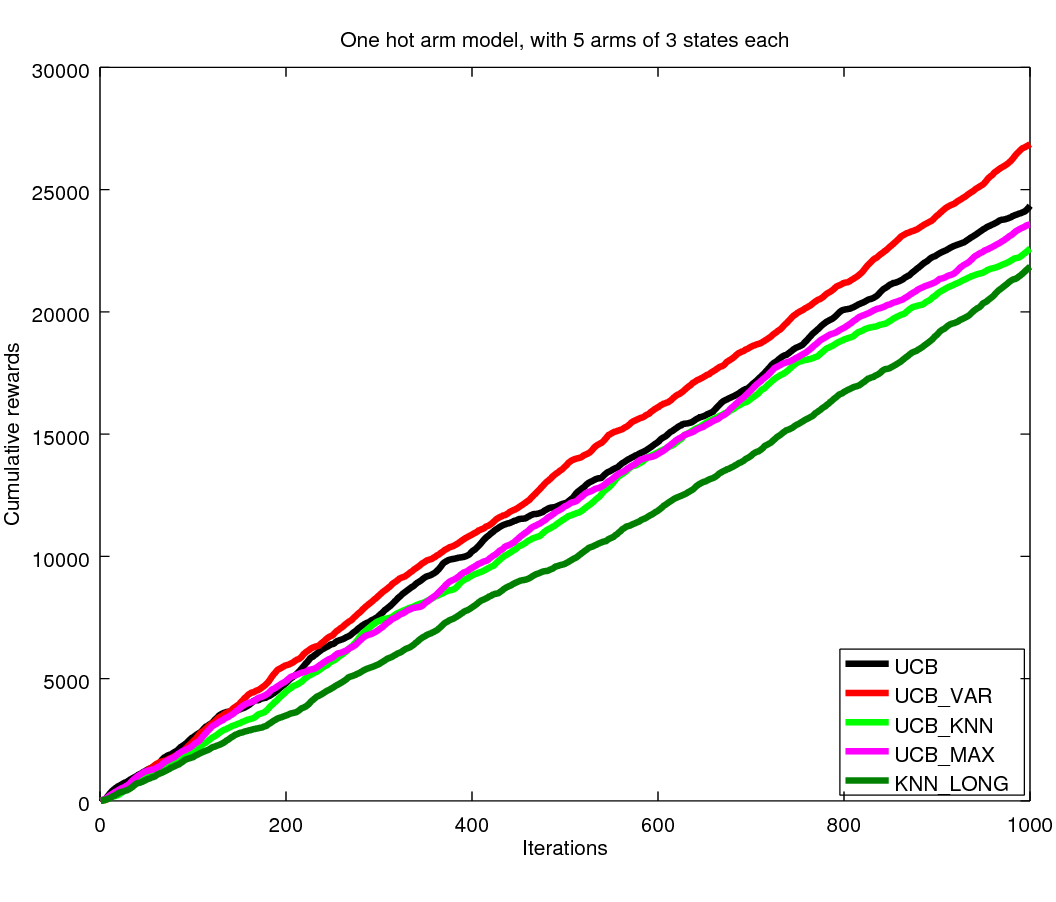
\includegraphics[width=1.0\textwidth]{begin_s_1000it.png}
		\caption{1000 first iterations (5*3, one)}
	\end{minipage}
	\hfill
	\begin{minipage}[b]{0.49\linewidth}
		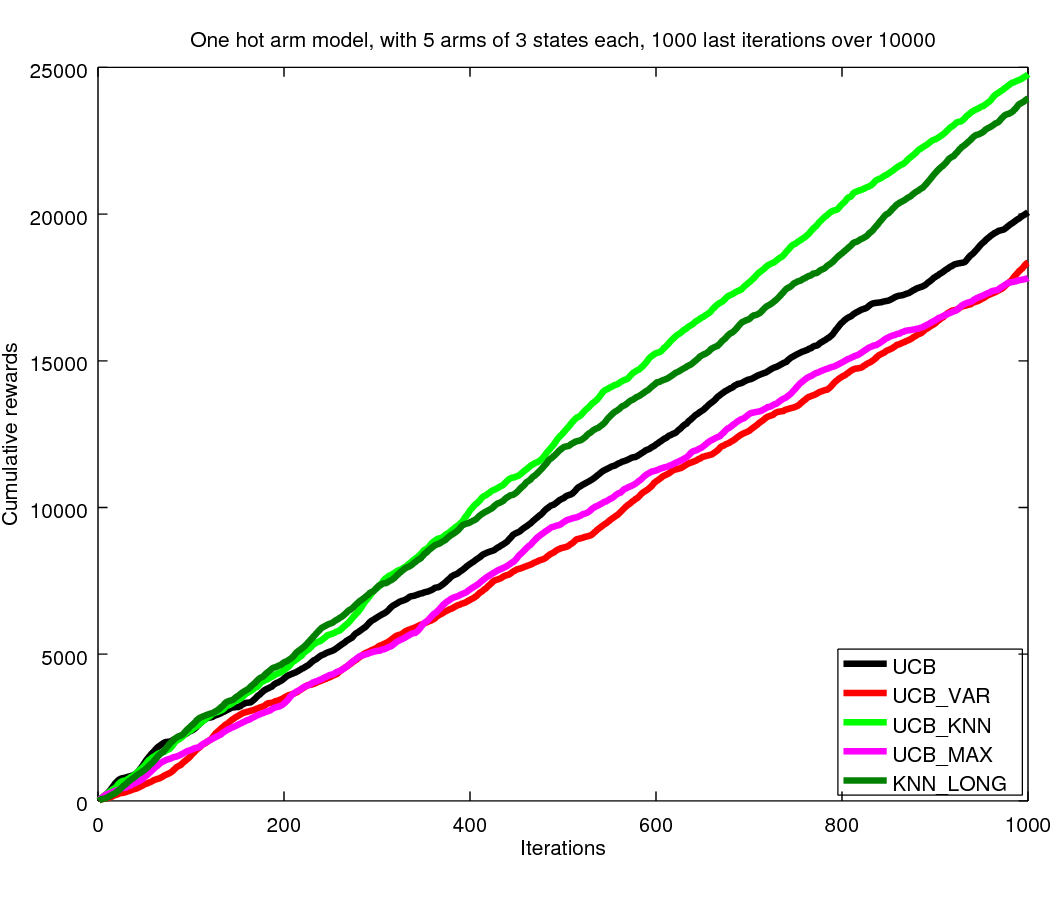
\includegraphics[width=1.0\textwidth]{last_s_1000it.png}
		\caption{1000 last iterations (5*3, one)}
	\end{minipage}
	\label{fig:f}
\end{figure}

We observe that the UCB algorithm performs better, indeed as there are more arms, it explores more so it finds more hot states and high rewards.

\clearpage
Eventually we tried the same version with several hot arms (5 runs each) : 

\begin{figure}[h]
	\begin{center}
		%\framebox[4.0in]{$\;$}
		%\fbox{\rule[-.5cm]{0cm}{4cm} \rule[-.5cm]{4cm}{0cm}}
		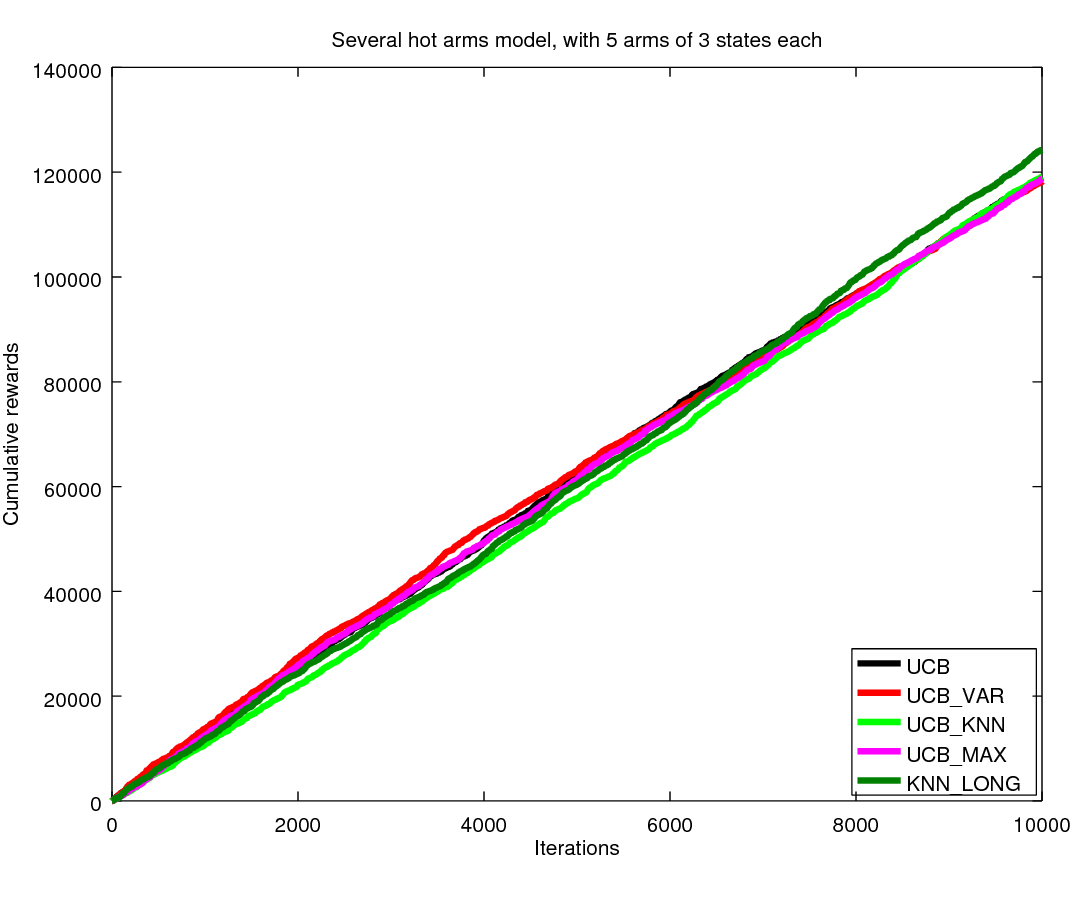
\includegraphics[width=1.0\textwidth]{all_ms_10000it.png}
	\end{center}
	\caption{All algorithms for 10000 iterations (5 arms * 3 states, several hot arms)}
\end{figure}

\begin{figure}[h]
	\begin{minipage}[b]{.49\linewidth}
		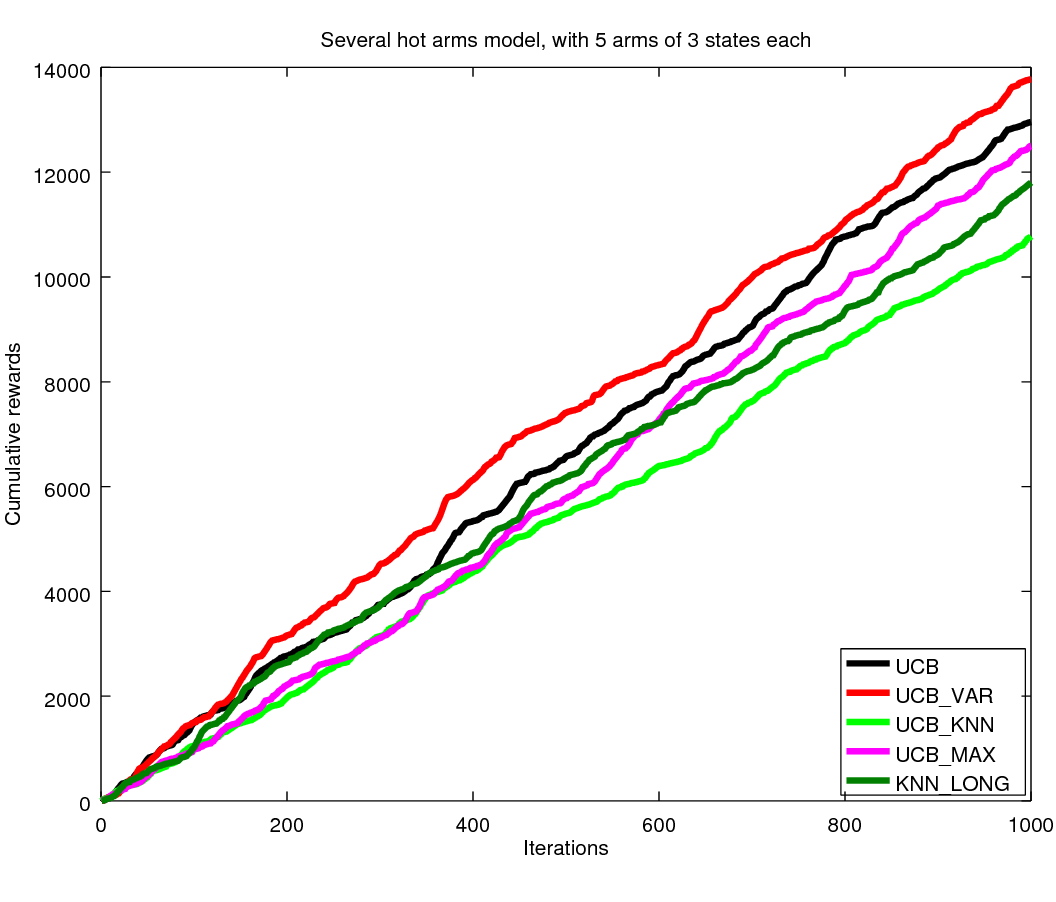
\includegraphics[width=1.0\textwidth]{begin_ms_1000it.png}
		\caption{1000 first iterations (5*3, several)}
	\end{minipage}
	\hfill
	\begin{minipage}[b]{0.49\linewidth}
		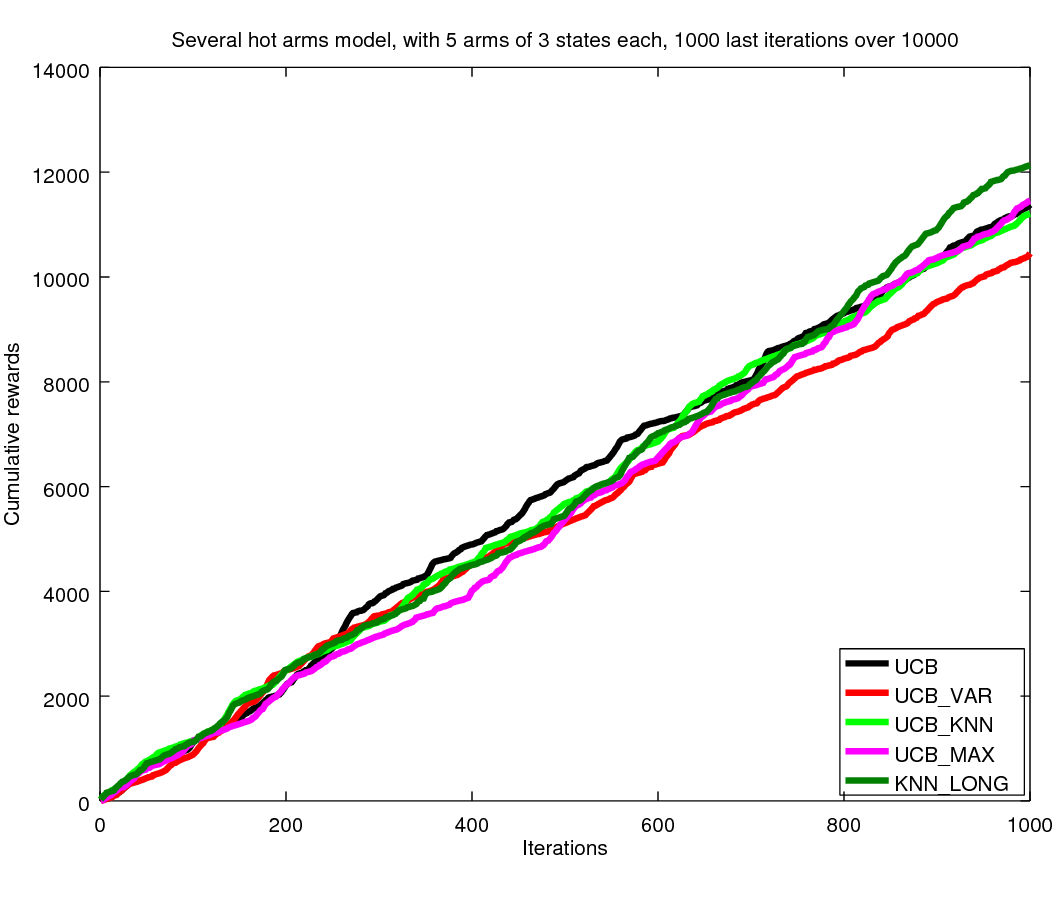
\includegraphics[width=1.0\textwidth]{last_ms_1000it.png}
		\caption{1000 last iterations (5*3, several)}
	\end{minipage}
	\label{fig:f}
\end{figure}

Here again the KNN\_LONG algorithm takes advantage for having a long term expectation calculation.

\clearpage
\section{Conclusion}


























\subsection{Style}

Papers to be submitted to NIPS 2015 must be prepared according to the
instructions presented here. Papers may be only up to eight pages long,
including figures. Since 2009 an additional ninth page \textit{containing only
cited references} is allowed. Papers that exceed nine pages will not be
reviewed, or in any other way considered for presentation at the conference.
%This is a strict upper bound.

Please note that this year we have introduced automatic line number generation
into the style file (for \LaTeXe and Word versions). This is to help reviewers
refer to specific lines of the paper when they make their comments. Please do
NOT refer to these line numbers in your paper as they will be removed from the
style file for the final version of accepted papers.

The margins in 2015 are the same as since 2007, which allow for $\approx 15\%$
more words in the paper compared to earlier years. We are also again using
double-blind reviewing. Both of these require the use of new style files.

Authors are required to use the NIPS \LaTeX{} style files obtainable at the
NIPS website as indicated below. Please make sure you use the current files and
not previous versions. Tweaking the style files may be grounds for rejection.

%% \subsection{Double-blind reviewing}

%% This year we are doing double-blind reviewing: the reviewers will not know
%% who the authors of the paper are. For submission, the NIPS style file will
%% automatically anonymize the author list at the beginning of the paper.

%% Please write your paper in such a way to preserve anonymity. Refer to
%% previous work by the author(s) in the third person, rather than first
%% person. Do not provide Web links to supporting material at an identifiable
%% web site.

%%\subsection{Electronic submission}
%%
%% \textbf{THE SUBMISSION DEADLINE IS June 5, 2015. SUBMISSIONS MUST BE LOGGED BY
%% 23:00, June 5, 2015, UNIVERSAL TIME}

%% You must enter your submission in the electronic submission form available at
%% the NIPS website listed above. You will be asked to enter paper title, name of
%% all authors, keyword(s), and data about the contact
%% author (name, full address, telephone, fax, and email). You will need to
%% upload an electronic (postscript or pdf) version of your paper.

%% You can upload more than one version of your paper, until the
%% submission deadline. We strongly recommended uploading your paper in
%% advance of the deadline, so you can avoid last-minute server congestion.
%%
%% Note that your submission is only valid if you get an e-mail
%% confirmation from the server. If you do not get such an e-mail, please
%% try uploading again.


\subsection{Retrieval of style files}

The style files for NIPS and other conference information are available on the World Wide Web at
\begin{center}
   \url{http://www.nips.cc/}
\end{center}
The file \verb+nips2015.pdf+ contains these
instructions and illustrates the
various formatting requirements your NIPS paper must satisfy. \LaTeX{}
users can choose between two style files:
\verb+nips15submit_09.sty+ (to be used with \LaTeX{} version 2.09) and
\verb+nips15submit_e.sty+ (to be used with \LaTeX{}2e). The file
\verb+nips2015.tex+ may be used as a ``shell'' for writing your paper. All you
have to do is replace the author, title, abstract, and text of the paper with
your own. The file
\verb+nips2015.rtf+ is provided as a shell for MS Word users.

The formatting instructions contained in these style files are summarized in
sections \ref{gen_inst}, \ref{headings}, and \ref{others} below.

%% \subsection{Keywords for paper submission}
%% Your NIPS paper can be submitted with any of the following keywords (more than one keyword is possible for each paper):

%% \begin{verbatim}
%% Bioinformatics
%% Biological Vision
%% Brain Imaging and Brain Computer Interfacing
%% Clustering
%% Cognitive Science
%% Control and Reinforcement Learning
%% Dimensionality Reduction and Manifolds
%% Feature Selection
%% Gaussian Processes
%% Graphical Models
%% Hardware Technologies
%% Kernels
%% Learning Theory
%% Machine Vision
%% Margins and Boosting
%% Neural Networks
%% Neuroscience
%% Other Algorithms and Architectures
%% Other Applications
%% Semi-supervised Learning
%% Speech and Signal Processing
%% Text and Language Applications

%% \end{verbatim}

\section{General formatting instructions}
\label{gen_inst}

The text must be confined within a rectangle 5.5~inches (33~picas) wide and
9~inches (54~picas) long. The left margin is 1.5~inch (9~picas).
Use 10~point type with a vertical spacing of 11~points. Times New Roman is the
preferred typeface throughout. Paragraphs are separated by 1/2~line space,
with no indentation.

Paper title is 17~point, initial caps/lower case, bold, centered between
2~horizontal rules. Top rule is 4~points thick and bottom rule is 1~point
thick. Allow 1/4~inch space above and below title to rules. All pages should
start at 1~inch (6~picas) from the top of the page.

%The version of the paper submitted for review should have ``Anonymous Author(s)'' as the author of the paper.

For the final version, authors' names are
set in boldface, and each name is centered above the corresponding
address. The lead author's name is to be listed first (left-most), and
the co-authors' names (if different address) are set to follow. If
there is only one co-author, list both author and co-author side by side.

Please pay special attention to the instructions in section \ref{others}
regarding figures, tables, acknowledgments, and references.

\section{Headings: first level}
\label{headings}

First level headings are lower case (except for first word and proper nouns),
flush left, bold and in point size 12. One line space before the first level
heading and 1/2~line space after the first level heading.

\subsection{Headings: second level}

Second level headings are lower case (except for first word and proper nouns),
flush left, bold and in point size 10. One line space before the second level
heading and 1/2~line space after the second level heading.

\subsubsection{Headings: third level}

Third level headings are lower case (except for first word and proper nouns),
flush left, bold and in point size 10. One line space before the third level
heading and 1/2~line space after the third level heading.

\section{Citations, figures, tables, references}
\label{others}

These instructions apply to everyone, regardless of the formatter being used.

\subsection{Citations within the text}

Citations within the text should be numbered consecutively. The corresponding
number is to appear enclosed in square brackets, such as [1] or [2]-[5]. The
corresponding references are to be listed in the same order at the end of the
paper, in the \textbf{References} section. (Note: the standard
\textsc{Bib\TeX} style \texttt{unsrt} produces this.) As to the format of the
references themselves, any style is acceptable as long as it is used
consistently.

As submission is double blind, refer to your own published work in the
third person. That is, use ``In the previous work of Jones et al.\ [4]'',
not ``In our previous work [4]''. If you cite your other papers that
are not widely available (e.g.\ a journal paper under review), use
anonymous author names in the citation, e.g.\ an author of the
form ``A.\ Anonymous''.


\subsection{Footnotes}

Indicate footnotes with a number\footnote{Sample of the first footnote} in the
text. Place the footnotes at the bottom of the page on which they appear.
Precede the footnote with a horizontal rule of 2~inches
(12~picas).\footnote{Sample of the second footnote}

\subsection{Figures}

All artwork must be neat, clean, and legible. Lines should be dark
enough for purposes of reproduction; art work should not be
hand-drawn. The figure number and caption always appear after the
figure. Place one line space before the figure caption, and one line
space after the figure. The figure caption is lower case (except for
first word and proper nouns); figures are numbered consecutively.

Make sure the figure caption does not get separated from the figure.
Leave sufficient space to avoid splitting the figure and figure caption.

You may use color figures.
However, it is best for the
figure captions and the paper body to make sense if the paper is printed
either in black/white or in color.
\begin{figure}[h]
\begin{center}
%\framebox[4.0in]{$\;$}
\fbox{\rule[-.5cm]{0cm}{4cm} \rule[-.5cm]{4cm}{0cm}}
\end{center}
\caption{Sample figure caption.}
\end{figure}

\subsection{Tables}

All tables must be centered, neat, clean and legible. Do not use hand-drawn
tables. The table number and title always appear before the table. See
Table~\ref{sample-table}.

Place one line space before the table title, one line space after the table
title, and one line space after the table. The table title must be lower case
(except for first word and proper nouns); tables are numbered consecutively.

\begin{table}[t]
\caption{Sample table title}
\label{sample-table}
\begin{center}
\begin{tabular}{ll}
\multicolumn{1}{c}{\bf PART}  &\multicolumn{1}{c}{\bf DESCRIPTION}
\\ \hline \\
Dendrite         &Input terminal \\
Axon             &Output terminal \\
Soma             &Cell body (contains cell nucleus) \\
\end{tabular}
\end{center}
\end{table}

\section{Final instructions}
Do not change any aspects of the formatting parameters in the style files.
In particular, do not modify the width or length of the rectangle the text
should fit into, and do not change font sizes (except perhaps in the
\textbf{References} section; see below). Please note that pages should be
numbered.

\section{Preparing PostScript or PDF files}

Please prepare PostScript or PDF files with paper size ``US Letter'', and
not, for example, ``A4''. The -t
letter option on dvips will produce US Letter files.

Fonts were the main cause of problems in the past years. Your PDF file must
only contain Type 1 or Embedded TrueType fonts. Here are a few instructions
to achieve this.

\begin{itemize}

\item You can check which fonts a PDF files uses.  In Acrobat Reader,
select the menu Files$>$Document Properties$>$Fonts and select Show All Fonts. You can
also use the program \verb+pdffonts+ which comes with \verb+xpdf+ and is
available out-of-the-box on most Linux machines.

\item The IEEE has recommendations for generating PDF files whose fonts
are also acceptable for NIPS. Please see
\url{http://www.emfield.org/icuwb2010/downloads/IEEE-PDF-SpecV32.pdf}

\item LaTeX users:

\begin{itemize}

\item Consider directly generating PDF files using \verb+pdflatex+
(especially if you are a MiKTeX user).
PDF figures must be substituted for EPS figures, however.

\item Otherwise, please generate your PostScript and PDF files with the following commands:
\begin{verbatim}
dvips mypaper.dvi -t letter -Ppdf -G0 -o mypaper.ps
ps2pdf mypaper.ps mypaper.pdf
\end{verbatim}

Check that the PDF files only contains Type 1 fonts.
%For the final version, please send us both the Postscript file and
%the PDF file.

\item xfig "patterned" shapes are implemented with
bitmap fonts.  Use "solid" shapes instead.
\item The \verb+\bbold+ package almost always uses bitmap
fonts.  You can try the equivalent AMS Fonts with command
\begin{verbatim}
\usepackage[psamsfonts]{amssymb}
\end{verbatim}
 or use the following workaround for reals, natural and complex:
\begin{verbatim}
\newcommand{\RR}{I\!\!R} %real numbers
\newcommand{\Nat}{I\!\!N} %natural numbers
\newcommand{\CC}{I\!\!\!\!C} %complex numbers
\end{verbatim}

\item Sometimes the problematic fonts are used in figures
included in LaTeX files. The ghostscript program \verb+eps2eps+ is the simplest
way to clean such figures. For black and white figures, slightly better
results can be achieved with program \verb+potrace+.
\end{itemize}
\item MSWord and Windows users (via PDF file):
\begin{itemize}
\item Install the Microsoft Save as PDF Office 2007 Add-in from
\url{http://www.microsoft.com/downloads/details.aspx?displaylang=en\&familyid=4d951911-3e7e-4ae6-b059-a2e79ed87041}
\item Select ``Save or Publish to PDF'' from the Office or File menu
\end{itemize}
\item MSWord and Mac OS X users (via PDF file):
\begin{itemize}
\item From the print menu, click the PDF drop-down box, and select ``Save
as PDF...''
\end{itemize}
\item MSWord and Windows users (via PS file):
\begin{itemize}
\item To create a new printer
on your computer, install the AdobePS printer driver and the Adobe Distiller PPD file from
\url{http://www.adobe.com/support/downloads/detail.jsp?ftpID=204} {\it Note:} You must reboot your PC after installing the
AdobePS driver for it to take effect.
\item To produce the ps file, select ``Print'' from the MS app, choose
the installed AdobePS printer, click on ``Properties'', click on ``Advanced.''
\item Set ``TrueType Font'' to be ``Download as Softfont''
\item Open the ``PostScript Options'' folder
\item Select ``PostScript Output Option'' to be ``Optimize for Portability''
\item Select ``TrueType Font Download Option'' to be ``Outline''
\item Select ``Send PostScript Error Handler'' to be ``No''
\item Click ``OK'' three times, print your file.
\item Now, use Adobe Acrobat Distiller or ps2pdf to create a PDF file from
the PS file. In Acrobat, check the option ``Embed all fonts'' if
applicable.
\end{itemize}

\end{itemize}
If your file contains Type 3 fonts or non embedded TrueType fonts, we will
ask you to fix it.

\subsection{Margins in LaTeX}

Most of the margin problems come from figures positioned by hand using
\verb+\special+ or other commands. We suggest using the command
\verb+\includegraphics+
from the graphicx package. Always specify the figure width as a multiple of
the line width as in the example below using .eps graphics
\begin{verbatim}
   \usepackage[dvips]{graphicx} ...
   \includegraphics[width=0.8\linewidth]{myfile.eps}
\end{verbatim}
or % Apr 2009 addition
\begin{verbatim}
   \usepackage[pdftex]{graphicx} ...
   \includegraphics[width=0.8\linewidth]{myfile.pdf}
\end{verbatim}
for .pdf graphics.
See section 4.4 in the graphics bundle documentation (\url{http://www.ctan.org/tex-archive/macros/latex/required/graphics/grfguide.ps})

A number of width problems arise when LaTeX cannot properly hyphenate a
line. Please give LaTeX hyphenation hints using the \verb+\-+ command.


\subsubsection*{Acknowledgments}

Use unnumbered third level headings for the acknowledgments. All
acknowledgments go at the end of the paper. Do not include
acknowledgments in the anonymized submission, only in the
final paper.

\subsubsection*{References}


\small{
[1] Auer, P., Cesa-Bianchi, N., & Fischer, P. (2002). Finite-time analysis of the multiarmed bandit problem. Machine learning, 47(2-3), 235-256.

[2] Agrawal, S., & Goyal, N. (2012, June). Analysis of Thompson Sampling for the Multi-armed Bandit Problem. In COLT (pp. 39-1).
}

\end{document}
